\documentclass[a4paper, 11pt]{article}
\usepackage{comment} % enables the use of multi-line comments (\ifx \fi) 
\usepackage{lipsum} %This package just generates Lorem Ipsum filler text. 
\usepackage{fullpage} % changes the margin
\usepackage{amsmath,amsfonts,amsthm} % Math packages
\usepackage{graphicx}
\usepackage{enumitem}
\setlist{nolistsep}
\usepackage{geometry}
\geometry{bottom=15mm}

\begin{document}
%Header-Make sure you update this information!!!!
\noindent
\large\textbf{Reinforcement Learning} \hfill %\textbf{FirstName LastName} \\
\normalsize Exercise 1 \hfill Team: Nico Ott, Lior, Hendrik Vloet \\
\hfill Lab Date: \today \\
\hfill Due Date: November 6, 2017
\section*{1 Introduction to RL}
\begin{itemize}
	\item \textbf{Model}: A model is an agent's internal representation of the environment that predicts its behavior, i.e. forecasts the environment's evolution, regarding an action of the agent.\\
	 A model may help a policy to find the best next action and it consists of 2 components:
	\begin{itemize}
		\item State-Transition model $\mathcal{P}$. It predicts the next state of the agent after executing an action. Formalized:
		\begin{flalign*}
			\mathcal{P} _{SS'} = \mathbb{P}  \left\lbrace S_{t+1}   = s' | S_t =s, A_t = a    \right\rbrace \\
		\end{flalign*}
		\item Reward model $\mathcal{R}^a _s$. It predicts the next expected (immediate) reward for the agent after performing some action, formalized:
		\begin{flalign*}
			\mathcal{R}^a _s = \mathbb{E} \lbrace R_{t+1} | S_t = s, A_t =a \rbrace \\
		\end{flalign*}
%		\vspace{-1.4cm}
%		\begin{figure}[hbpt!]
%		\centering
%		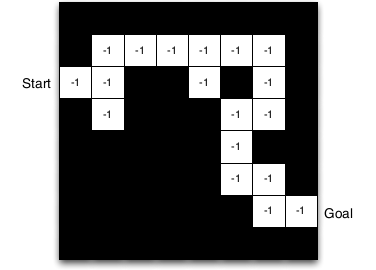
\includegraphics[width=0.5\textwidth,height=4cm]{example_model}
%		\caption{Example for a model. The grid layout represents the transition model(which can be imperfect; compare to the full grid in D.Silvers lecture) $\mathcal{P}^a _{ss'}$ and the numbers represent the immediate reward $\mathcal{R}^a _s$ from each state $s$ (in this case the same for every action $a$). Picture taken from David Silvers Reinforcement Learning Lecture.}
%		\end{figure}
	\end{itemize}
    \item \textbf{Policy}: the policy is the behavior of the agent, i.e. it is a mapping function from state to an action. Or in other words: it is a strategy how the agent will choose its next action, taking into account in which state it is. Nevertheless, a policy does not guarantee optimal performance, since it just represents one possible behavior of the agent out of infinitely many. Briefly, it can be good or bad and thus increase or decrease performance.\\
     We can divide them into two overall classes:
    \begin{itemize}
    	\item deterministic policy, where the outcome of an evaluation of the state is exactly known: \\ 
    	\begin{align*}
    	a = \pi(s)
    	\end{align*}
    	\item stochastic policy, where the outcome of an evaluation of the state is not exactly known but can be described with the help of probabilistic calculus:\\
    	\begin{align*}
    		\pi( a | s) = \mathbb{P}(A_t =a | S_t = s)
    	\end{align*}
    \end{itemize}
    \vspace{0.5cm}
    \item \textbf{Value-function}: predicts the future reward of the agent and is used to evaluate the goodness/badness of states, i.e. the value function can be used to pick actions, depending of the outcome. The value functions "unrolls" future possible rewards under some policy $\pi$:\\
    $v_{\pi} ^{(s)} = \mathbb{E}_{\pi} \lbrace R_{t+1}+ \gamma R_{t+2} + \gamma ^2 R_{t+3}+... | S_t = s \rbrace$
\end{itemize}
\clearpage


\section*{2 GYM}

\lipsum[1]

\end{document}
